%%
%% This is file `sample-sigplan.tex',
%% generated with the docstrip utility.
%%
%% The original source files were:
%%
%% samples.dtx  (with options: `all,proceedings,bibtex,sigplan')
%% 
%% IMPORTANT NOTICE:
%% 
%% For the copyright see the source file.
%% 
%% Any modified versions of this file must be renamed
%% with new filenames distinct from sample-sigplan.tex.
%% 
%% For distribution of the original source see the terms
%% for copying and modification in the file samples.dtx.
%% 
%% This generated file may be distributed as long as the
%% original source files, as listed above, are part of the
%% same distribution. (The sources need not necessarily be
%% in the same archive or directory.)
%%
%%
%% Commands for TeXCount
%TC:macro \cite [option:text,text]
%TC:macro \citep [option:text,text]
%TC:macro \citet [option:text,text]
%TC:envir table 0 1
%TC:envir table* 0 1
%TC:envir tabular [ignore] word
%TC:envir displaymath 0 word
%TC:envir math 0 word
%TC:envir comment 0 0
%%
%% The first command in your LaTeX source must be the \documentclass
%% command.
%%
%% For submission and review of your manuscript please change the
%% command to \documentclass[manuscript, screen, review]{acmart}.
%%
%% When submitting camera ready or to TAPS, please change the command
%% to \documentclass[sigconf]{acmart} or whichever template is required
%% for your publication.
%%
%%
\documentclass[sigplan,screen]{acmart}

% \documentclass[sigconf,screen,final,nonacm]{acmart}

\usepackage{graphicx}
\usepackage{hyperref}
\usepackage{algorithm}
\usepackage{algpseudocode}
\usepackage{tikz}
\usetikzlibrary{trees,positioning,shapes,arrows,calc,shapes.geometric,arrows.meta} % Added shapes.geometric, arrows.meta
\usepackage{listings} % For code listings
\usepackage{multirow} % For tables
\usepackage{xcolor} % Required for background color
\usepackage{tabularx} % For better table column width management

\newcommand{\circled}[1]{%
  \tikz[baseline=(char.base)]{
    \node[shape=circle, fill=black, text=white, inner sep=1pt, minimum size=1.5em] (char) {#1};
  }%
}



% Define a light gray color
% \definecolor{codegray}{gray}{0.95}

% \lstset{
%   backgroundcolor=\color{codegray}, % Light gray background
%   basicstyle=\footnotesize\ttfamily,
%   breaklines=true,
%   frame=tb, % Top and bottom frame lines
%   framesep=3pt, % Padding around frame
%   showstringspaces=false,
%   keywordstyle=\color{blue}, % Standard blue keywords
%   commentstyle=\color{green!60!black}, % Standard green comments
%   stringstyle=\color{purple}, % Standard purple strings
%   numbers=left, % Add line numbers
%   numberstyle=\tiny\color{gray}, % Style for line numbers
%   tabsize=2, % Set tab size
%   captionpos=b % Place caption below listing
% }

% Enhanced original code listing style
\definecolor{codegray}{RGB}{245, 246, 248}  % Slightly more refined light gray

\lstset{
  backgroundcolor=\color{codegray},    % Light gray background
  basicstyle=\footnotesize\ttfamily,   % Keep original font style
  breaklines=true,                     % Line wrapping
  frame=tb,                            % Keep top and bottom frame lines
  framesep=3pt,                        % Padding around frame
  showstringspaces=false,              % Don't show spaces in strings
  keywordstyle=\color{blue}\bfseries,  % Bold blue keywords
  commentstyle=\color{green!60!black}, % Keep original green comments
  stringstyle=\color{purple},          % Keep original purple strings
  numbers=left,                        % Line numbers on left
  numberstyle=\tiny\color{gray},       % Style for line numbers
  tabsize=2,                           % Tab size
  captionpos=b,                        % Caption below listing
  xleftmargin=8pt,                     % Add left margin
  numbersep=5pt,                       % Spacing between numbers and code
  framexleftmargin=8pt,                % Extend frame to cover line numbers
  aboveskip=\medskipamount,            % Space above listing
  belowskip=\medskipamount,            % Space below listing
  columns=flexible,                    % Better spacing
  keepspaces=true,                     % Keep indentation
  upquote=true                         % Straight quotes
}

%%
%% \BibTeX command to typeset BibTeX logo in the docs
\AtBeginDocument{%
  \providecommand\BibTeX{{%
    Bib\TeX}}}

%% Rights management information.  This information is sent to you
%% when you complete the rights form.  These commands have SAMPLE
%% values in them; it is your responsibility as an author to replace
%% the commands and values with those provided to you when you
%% complete the rights form.
\setcopyright{acmlicensed}
\copyrightyear{2024} % Assuming current year for now
\acmYear{2024} % Assuming current year for now
\acmDOI{XXXXXXX.XXXXXXX} % Placeholder DOI
%% These commands are for a PROCEEDINGS abstract or report.
\acmConference[Conference Acronym 'XX]{Make sure to enter the correct
  conference title from your rights confirmation email}{Date}{Location} % Placeholder conference details
%%
%%  Uncomment \acmBooktitle if the title of the proceedings is different
%%  from ``Proceedings of ...''!
%%
%%\acmBooktitle{Woodstock '18: ACM Symposium on Neural Gaze Detection,
%%  June 03--05, 2018, Woodstock, NY}
\acmISBN{978-1-4503-XXXX-X/24/05} % Placeholder ISBN


%%
%% Submission ID.
%% Use this when submitting an article to a sponsored event. You'll
%% receive a unique submission ID from the organizers
%% of the event, and this ID should be used as the parameter to this command.
%%\acmSubmissionID{123-A56-BU3}

%%
%% For managing citations, it is recommended to use bibliography
%% files in BibTeX format.
%%
%% You can then either use BibTeX with the ACM-Reference-Format style,
%% or BibLaTeX with the acmnumeric or acmauthoryear sytles, that include
%% support for advanced citation of software artefact from the
%% biblatex-software package, also separately available on CTAN.
%%
%% Look at the sample-*-biblatex.tex files for templates showcasing
%% the biblatex styles.
%%

%%
%% The majority of ACM publications use numbered citations and
%% references.  The command \citestyle{authoryear} switches to the
%% "author year" style.
%%
%% If you are preparing content for an event
%% sponsored by ACM SIGGRAPH, you must use the "author year" style of
%% citations and references.
%% Uncommenting
%% the next command will enable that style.
%%\citestyle{acmauthoryear}


%%
%% end of the preamble, start of the body of the document source.
\begin{document}

%%
%% The "title" command has an optional parameter,
%% allowing the author to define a "short title" to be used in page headers.
\title[Hardware Trojan Detection using GNNs on ASTs]{Hardware Trojan Detection Using Graph Neural Networks: An AST-based GCN Approach}

%%
%% The "author" command and its associated commands are used to define
%% the authors and their affiliations.
%% Of note is the shared affiliation of the first two authors, and the
%% "authornote" and "authornotemark" commands
%% used to denote shared contribution to the research.
\author{Md Omar Faruque} % Placeholder Author
\email{xxxxx@example.com} % Placeholder Email
\affiliation{%
  \institution{xxxxxx} % Placeholder Institution
  \city{xxxx}
  \state{xxxx}
  \country{xxxx}
}
% Add more authors as needed

%%
%% By default, the full list of authors will be used in the page
%% headers. Often, this list is too long, and will overlap
%% other information printed in the page headers. This command allows
%% the author to define a more concise list
%% of authors' names for this purpose.
\renewcommand{\shortauthors}{Your Name et al.} % Placeholder short authors

%%
%% The abstract is a short summary of the work to be presented in the
%% article.
\begin{abstract}
Hardware Trojans (HTs) pose a significant threat to the security and integrity of integrated circuits. Detecting these malicious modifications, especially at the Register-Transfer Level (RTL), is a challenging task. This report presents a learning journey on hardware Trojan detection using Graph Convolutional Networks (GCNs) applied to Abstract Syntax Tree (AST) representations of hardware designs. We leverage the structural and semantic information captured by ASTs to train a GCN model capable of distinguishing between Trojan-free and Trojan-infected designs. Our methodology involves parsing Verilog code into ASTs, extracting relevant features, and training a GCN model on a processed dataset derived from TrustHub benchmarks. Experimental results demonstrate the effectiveness of our approach, achieving a high F1 score in detecting various types of hardware Trojans.
\end{abstract}

%%
%% The code below is generated by the tool at http://dl.acm.org/ccs.cfm.
%% Please copy and paste the code instead of the example below.
%%

\begin{CCSXML}
<ccs2012>
   <concept>
       <concept_id>10002978.10003006.10003013</concept_id>
       <concept_desc>Security and privacy~Embedded systems security</concept_desc>
       <concept_significance>500</concept_significance>
       </concept>
   <concept>
       <concept_id>10010520.10010521.10010542.10010294</concept_id>
       <concept_desc>Computer systems organization~Hardware-software codesign</concept_desc>
       <concept_significance>300</concept_significance>
       </concept>
   <concept>
       <concept_id>10010147.10010257.10010293.10010294</concept_id>
       <concept_desc>Computing methodologies~Neural networks</concept_desc>
       <concept_significance>300</concept_significance>
       </concept>
 </ccs2012>
\end{CCSXML}

\ccsdesc[500]{Security and privacy~Embedded systems security}
\ccsdesc[300]{Computer systems organization~Hardware-software codesign}
\ccsdesc[300]{Computing methodologies~Neural networks}

%%
%% Keywords. The author(s) should pick words that accurately describe
%% the work being presented. Separate the keywords with commas.
\keywords{Hardware security, Trojan detection, graph neural networks, abstract syntax tree, GCN, hardware verification, RTL}

%% A "teaser" image appears between the author and affiliation
%% information and the body of the document, and typically spans the
%% page.
% \begin{teaserfigure}
%   \includegraphics[width=\textwidth]{sampleteaser}
%   \caption{Seattle Mariners at Spring Training, 2010.}
%   \Description{Enjoying the baseball game from the third-base
%   seats. Ichiro Suzuki preparing to bat.}
%   \label{fig:teaser}
% \end{teaserfigure}

% \received{20 February 2007}
% \received[revised]{12 March 2009}
% \received[accepted]{5 June 2009}

%%
%% This command processes the author and affiliation and title
%% information and builds the first part of the formatted document.
\maketitle

\section{Introduction}
The increasing complexity and globalization of the integrated circuit (IC) supply chain have raised significant concerns about hardware security. Hardware Trojans (HTs), malicious modifications intentionally inserted into ICs during design or fabrication, pose a severe threat to the trustworthiness of electronic systems. These Trojans can lead to various detrimental effects, including information leakage, denial of service, or complete system failure. Detecting HTs, particularly at the Register-Transfer Level (RTL) where designs are often shared with untrusted third parties, is a critical yet challenging task.

Traditional HT detection methods, such as logic testing and side-channel analysis, often struggle with the stealthy nature of modern Trojans, which can be small, cleverly hidden, and triggered by rare conditions. Machine learning (ML) techniques have emerged as a promising alternative, offering the potential to learn patterns indicative of Trojans from large datasets of hardware designs. Among ML approaches, Graph Neural Networks (GNNs) are particularly well-suited for analyzing graph-structured data, such as hardware circuits.

This report proposes an approach for hardware Trojan detection by applying Graph Convolutional Networks (GCNs) to Abstract Syntax Tree (AST) representations of RTL Verilog code. ASTs capture rich structural and semantic information from the source code, providing a more detailed representation than traditional circuit graphs. By leveraging GCNs to learn from these ASTs, our method aims to effectively identify subtle differences between Trojan-free and Trojan-infected designs.

The main contributions of this work are:
\begin{enumerate}
    \item The application of GCNs for classifying hardware designs as Trojan-free or Trojan-infected based on their AST representations.
    \item An empirical evaluation of the proposed approach on a processed dataset derived from TrustHub benchmarks, demonstrating its effectiveness in detecting various types of hardware Trojans.
\end{enumerate}

The remainder of this report is organized as follows: Section 3 discusses the methodology, including the theoretical framework and the proposed GCN-on-AST approach. Section 4 details the experimental setup, including the dataset, implementation details, and evaluation metrics. Section 5 presents and analyzes the experimental results. Section 6 discusses the key findings and limitations of our work. Finally, Section 7 concludes the report and outlines future research directions.

\section{Methodology}
\subsection{Theoretical Framework}
\subsubsection{Graph Representation for Hardware Designs}
Hardware designs, particularly at the RTL, can be naturally represented as graphs. Nodes in such graphs can represent various hardware elements like modules, instances, wires, or operations, while edges can represent connections or dependencies between these elements. Graph-based representations allow for the application of powerful graph learning algorithms.

\subsubsection{Abstract Syntax Trees (ASTs)}
An Abstract Syntax Tree (AST) is a tree representation of the abstract syntactic structure of source code~\cite{aho2007compilers}. Each node in an AST denotes a construct occurring in the source code. Unlike concrete syntax trees, ASTs do not represent every detail appearing in the real syntax, but rather focus on the structural and semantic aspects~\cite{necula2002cil}. For hardware description languages (HDLs) like Verilog, an AST can capture the hierarchical structure of modules, instances, assignments, control flow statements, and expressions. This detailed representation is beneficial for identifying subtle malicious modifications~\cite{yamaguchi2014modeling}.

Algorithm~\ref{alg:ast_generation} outlines the general process for generating an AST from Verilog code.

\begin{algorithm}
\caption{AST Generation from Verilog Code}
\label{alg:ast_generation}
\begin{algorithmic}[1]
\Procedure{GenerateAST}{VerilogFile}
    \State $Source \gets \text{Read}(VerilogFile)$
    \State $Tokens \gets \text{LexicalAnalysis}(Source)$
    \State $ParseTree \gets \text{SyntaxAnalysis}(Tokens)$
    \State $AST_{root} \gets \text{AbstractParseTree}(ParseTree)$
    \Function{BuildGraph}{$Node, ParentNode, Graph$}
        \State $Graph.\text{AddNode}(Node.\text{id}, \text{type}=Node.\text{type}, \text{attributes}=...)$
        \If{$ParentNode \neq \text{null}$}
            \State $Graph.\text{AddEdge}(ParentNode.\text{id}, Node.\text{id})$
        \EndIf
        \ForAll{$Child \in Node.\text{children}$}
            \State BuildGraph($Child, Node, Graph$)
        \EndFor
    \EndFunction
    \State $Graph_{AST} \gets \text{InitializeGraph}()$
    \State BuildGraph($AST_{root}, \text{null}, Graph_{AST}$)
    \State \textbf{return} $Graph_{AST}$
\EndProcedure
\end{algorithmic}
\end{algorithm}

Consider the following simple Verilog module for a 4-bit counter as a toy example:
% Use standard lstlisting with updated style
\begin{lstlisting}[language=Verilog, caption=A simple 4-bit counter in Verilog., label=lst:counter_verilog]
module counter (
  input clk,
  output reg [3:0] count
);
  always @(posedge clk) begin
    count <= count + 1;
  end
endmodule
\end{lstlisting}

Figure~\ref{fig:ast_example} illustrates a simplified AST for this `counter` module (Listing~\ref{lst:counter_verilog}). The AST captures the module definition, its ports, and the `always` block with the increment operation. Figure~\ref{fig:ast_process} shows the general process of generating this AST graph representation from the source code.

\begin{figure}[h]
\centering
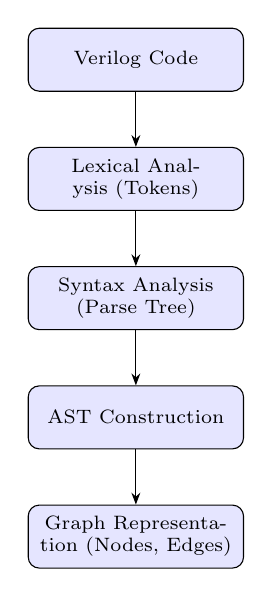
\begin{tikzpicture}[
    node distance=7mm and 10mm, % Vertical and horizontal distances
    block/.style={rectangle, draw, fill=blue!10, text centered, rounded corners, minimum height=8mm, text width=25mm, font=\scriptsize},
    arrow/.style={draw, -{Stealth[length=1.5mm]}} % Use Stealth arrow tip
]
    % Nodes
    \node (verilog) [block] {Verilog Code};
    \node (lexer) [block, below=of verilog] {Lexical Analysis (Tokens)};
    \node (parser) [block, below=of lexer] {Syntax Analysis (Parse Tree)};
    \node (ast) [block, below=of parser] {AST Construction};
    \node (graph) [block, below=of ast] {Graph Representation (Nodes, Edges)};

    % Connections
    \path [arrow] (verilog) -- (lexer);
    \path [arrow] (lexer) -- (parser);
    \path [arrow] (parser) -- (ast);
    \path [arrow] (ast) -- (graph);

\end{tikzpicture}
\caption{AST Graph Generation Process.}
\label{fig:ast_process}
\end{figure}


\begin{figure}[htbp] % Changed placement specifier
\centering
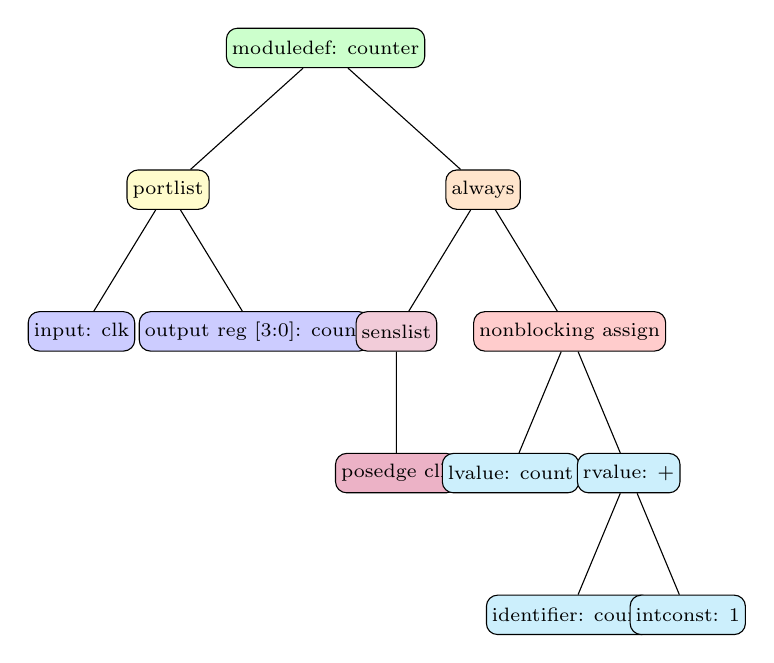
\begin{tikzpicture}[
    level distance=1.2cm, % Adjusted for better spacing
    level 1/.style={sibling distance=40mm, level distance=18mm},
    level 2/.style={sibling distance=22mm, level distance=18mm},
    level 3/.style={sibling distance=15mm, level distance=18mm},
    every node/.style={draw, rounded corners, font=\scriptsize, text centered, minimum height=5mm, inner sep=2pt}, % General node style
    module/.style={fill=green!20}, % ModuleDef
    portlist/.style={fill=yellow!20}, % Portlist
    port/.style={fill=blue!20}, % Port
    alwaysblk/.style={fill=orange!20}, % Always
    senslist/.style={fill=purple!20}, % Senslist
    event/.style={fill=purple!30}, % Posedge, Negedge
    stmt/.style={fill=red!20}, % Statement (Nonblocking)
    expr/.style={fill=cyan!20} % Expression
]
\node[module] {moduledef: counter}
    child { node[portlist] {portlist}
        child { node[port] {input: clk} }
        child { node[port] {output reg [3:0]: count} } % More descriptive
    }
    child { node[alwaysblk] {always}
        child { node[senslist] {senslist}
            child { node[event] {posedge clk} }
        }
        child { node[stmt] {nonblocking assign} % More descriptive
            child { node[expr] {lvalue: count} }
            child { node[expr] {rvalue: +}
                child { node[expr] {identifier: count} }
                child { node[expr] {intconst: 1} }
            }
        }
    };
\end{tikzpicture}
\caption{Simplified AST for the 4-bit counter module (Listing~\ref{lst:counter_verilog}).}
\label{fig:ast_example}
\end{figure}

During the parsing of various Verilog files in the dataset, a dictionary of AST node types is generated. This typically includes over 45 unique node types such as `ModuleDef`, `Portlist`, `Decl` (for declarations like `input`, `output`, `reg`, `wire`), `InstanceList`, `Assign`, `Always`, `IfStatement`, `CaseStatement`, `BlockingSubstitution`, `NonblockingSubstitution`, `Identifier`, `IntConst`, various operators (`Plus`, `Minus`, `And`, `Or`, `Xor`), `Partselect`, `Concat`, etc. Each unique node type is assigned an integer ID, which is then used for feature encoding.

\subsubsection{Graph Neural Networks (GNNs)}
Graph Neural Networks (GNNs) are a class of deep learning models designed to perform inference on data described by graphs~\cite{zhou2020graph}. GNNs operate by iteratively aggregating information from a node's neighbors to update its representation (embedding). This message-passing mechanism allows GNNs to learn complex patterns and relationships within graph-structured data~\cite{wu2020comprehensive}.

\subsubsection{Graph Convolutional Networks (GCNs)}
Graph Convolutional Networks (GCNs)~\cite{kipf2017semi} are a specific type of GNN that generalizes the concept of convolution from regular grids (like images) to irregular graph structures. A common GCN layer updates the feature vector of a node $v_i$ by aggregating the feature vectors of its neighbors $\mathcal{N}(i)$, often followed by a linear transformation and a non-linear activation function~\cite{hamilton2017inductive}. The layer-wise propagation rule for a GCN can be expressed as:
\begin{equation} \label{eq:gcn}
H^{(l+1)} = \sigma\left(\tilde{D}^{-\frac{1}{2}}\tilde{A}\tilde{D}^{-\frac{1}{2}}H^{(l)}W^{(l)}\right)
\end{equation}
where $H^{(l)} \in \mathbb{R}^{N \times F^{(l)}}$ is the matrix of node activations in layer $l$ (with $H^{(0)}=X$ being the initial node features, $N$ nodes, $F^{(l)}$ features per node in layer $l$), $W^{(l)} \in \mathbb{R}^{F^{(l)} \times F^{(l+1)}}$ is a layer-specific trainable weight matrix. $\sigma(\cdot)$ is an activation function (e.g., ReLU). $\tilde{A} = A + I_N$ is the adjacency matrix of the graph $G$ with added self-loops (where $I_N$ is the identity matrix), and $\tilde{D}$ is the diagonal degree matrix of $\tilde{A}$, i.e., $\tilde{D}_{ii} = \sum_j \tilde{A}_{ij}$. The term $\tilde{D}^{-\frac{1}{2}}\tilde{A}\tilde{D}^{-\frac{1}{2}}$ serves as a symmetric normalization of the adjacency matrix.

\subsection{Proposed Approach}
\subsubsection{AST-based Hardware Representation}
Our approach begins by parsing RTL Verilog files into ASTs, as outlined in Algorithm~\ref{alg:ast_generation}. Each node in the AST represents a syntactic construct from the Verilog code (e.g., module definition, port declaration, assignment, instance). Edges in the AST represent the hierarchical relationships between these constructs (e.g., a module node has children nodes representing its ports, declarations, and instances).

\subsubsection{Feature Extraction}
For each node in the AST, a feature vector is constructed to capture its characteristics and context within the hardware design. The features used in this work include:
\circled{1} \textbf{Node Type Encoding}: The type of the AST node (e.g., `ModuleDef`, `Assign`, `Identifier`) is represented using one-hot encoding. Given that over 45 unique node types were discovered across the dataset, a vector of approximately 50 dimensions is used for this encoding, where the dimension corresponding to the node's type is set to 1 and others to 0.
\circled{2} \textbf{Node Depth}: An integer representing the depth of the node in the AST, indicating its hierarchical level.
\circled{3} \textbf{Number of Children}: An integer count of the direct children of the node, reflecting its local complexity or fan-out in the tree structure.
\circled{4} \textbf{Average Child Type ID}: A float value calculated as the average of the numerical IDs of its children's types. This feature provides contextual information about the node's immediate descendants.

Combining these, each node is represented by a feature vector of 50+ dimensions (e.g., 50 for one-hot type encoding + 3 for structural features). These features aim to capture both the specific function of a node and its structural role within the AST.

\subsubsection{GCN Architecture for Trojan Detection}
The core of our detection methodology is a GCN model specifically designed to process the AST graphs. The overall framework is depicted in Figure~\ref{fig:overall_framework}, and the detailed GCN architecture is shown in Figure~\ref{fig:gcn_architecture}.

% \begin{figure}[h] % Reverted placement and layout
% \centering
% \begin{tikzpicture}[
%     node distance=6mm and 8mm, % Original distances
%     block/.style={rectangle, draw, fill=blue!10, text centered, rounded corners, minimum height=7mm, text width=20mm, font=\tiny}, % Original size
%     arrow/.style={draw, -{Stealth[length=1.2mm]}} % Original arrow tip
% ]
%     % Nodes - Arranged horizontally again
%     \node (verilog) [block] {Input Verilog};
%     \node (astgen) [block, right=of verilog] {AST Gen. \& Features}; % Shorter text
%     \node (gcnmodel) [block, right=of astgen] {GCN Model};
%     \node (output) [block, right=of gcnmodel] {Classification}; % Shorter text

%     % Connections
%     \path [arrow] (verilog) -- (astgen);
%     \path [arrow] (astgen) -- node[above, font=\tiny] {Graph} (gcnmodel); % Shorter text
%     \path [arrow] (gcnmodel) -- node[above, font=\tiny] {Prob.} (output); % Shorter text

% \end{tikzpicture}
% \caption{Overall Proposed Framework for Trojan Detection.}
% \label{fig:overall_framework}
% \end{figure}

% \begin{figure}[htbp] % Changed placement specifier
% \centering
% \begin{tikzpicture}[
%     node distance=8mm and 5mm, % Adjusted distances for single column
%     block/.style={rectangle, draw, fill=blue!10, text centered, rounded corners, minimum height=8mm, text width=25mm, font=\scriptsize}, % Adjusted width
%     gcn/.style={rectangle, draw, fill=green!10, text centered, rounded corners, minimum height=8mm, text width=25mm, font=\scriptsize}, % Adjusted width
%     pool/.style={rectangle, draw, fill=yellow!10, text centered, rounded corners, minimum height=8mm, text width=25mm, font=\scriptsize}, % Adjusted width
%     mlp/.style={rectangle, draw, fill=cyan!10, text centered, rounded corners, minimum height=8mm, text width=25mm, font=\scriptsize}, % Adjusted width
%     output/.style={rectangle, draw, fill=red!10, text centered, rounded corners, minimum height=8mm, text width=25mm, font=\scriptsize}, % Adjusted width
%     ops/.style={ellipse, draw, fill=orange!10, minimum size=6mm, font=\tiny}, % Smaller ops nodes
%     line/.style={draw, -{Stealth[length=1.5mm]}} % Use Stealth arrow tip
% ]
%     % Nodes - Arranged vertically
%     \node (input) [block] {Input AST Graph (N nodes, F features)};
%     \node (gcn1) [gcn, below=of input] {GCN Layer 1 (64 units)};
%     \node (ops1) [ops, below=2mm of gcn1] {ReLU + Dropout}; % Ops below
%     \node (gcn2) [gcn, below=8mm of ops1] {GCN Layer 2 (64 units)}; % Increased distance
%     \node (ops2) [ops, below=2mm of gcn2] {ReLU + Dropout}; % Ops below
%     \node (pooling) [pool, below=8mm of ops2] {Global Mean Pooling}; % Increased distance
%     \node (mlp_block) [mlp, below=of pooling] {MLP Classifier};
%     \node (ops3) [ops, below=2mm of mlp_block] {Sigmoid}; % Ops below
%     \node (output_node) [output, below=8mm of ops3] {Output Probability}; % Increased distance

%     % Connections
%     \path [line] (input) -- node[right, font=\tiny] {$H^{(0)}$} (gcn1);
%     \path [line] (gcn1) -- (ops1);
%     \path [line] (ops1) -- node[right, font=\tiny] {$H^{(1)}$} (gcn2);
%     \path [line] (gcn2) -- (ops2);
%     \path [line] (ops2) -- node[right, font=\tiny] {$H^{(2)}$} (pooling);
%     \path [line] (pooling) -- node[right, font=\tiny] {Graph Emb.} (mlp_block);
%     \path [line] (mlp_block) -- (ops3);
%     \path [line] (ops3) -- (output_node);

% \end{tikzpicture}
% \caption{Detailed GCN Model Architecture (Single Column).}
% \label{fig:gcn_architecture}
% \end{figure}

% First figure - Framework diagram converted to vertical layout
\begin{figure}[htbp]
  \centering
  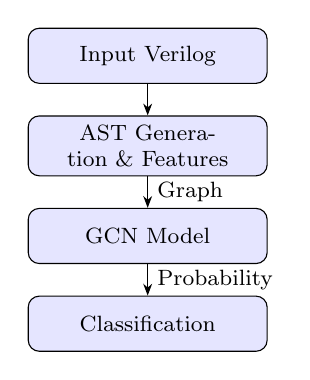
\begin{tikzpicture}[
      node distance=4mm, % Reduced vertical distance
      block/.style={rectangle, draw, fill=blue!10, text centered, rounded corners, minimum height=7mm, text width=28mm, font=\footnotesize} % Wider blocks
  ]
      % Nodes - Arranged vertically
      \node (verilog) [block] {Input Verilog};
      \node (astgen) [block, below=of verilog] {AST Generation \& Features}; 
      \node (gcnmodel) [block, below=of astgen] {GCN Model};
      \node (output) [block, below=of gcnmodel] {Classification}; 
  
      % Connections with straight arrows
      \draw[-{Stealth[length=1.5mm]}] (verilog) -- (astgen);
      \draw[-{Stealth[length=1.5mm]}] (astgen) -- node[right, font=\footnotesize] {Graph} (gcnmodel);
      \draw[-{Stealth[length=1.5mm]}] (gcnmodel) -- node[right, font=\footnotesize] {Probability} (output);
  \end{tikzpicture}
  \caption{Overall Proposed Framework for Trojan Detection.}
  \label{fig:overall_framework}
  \end{figure}
  
  % Second figure - GCN Architecture already vertical, but optimized for single column
  \begin{figure}[htbp]
  \centering
  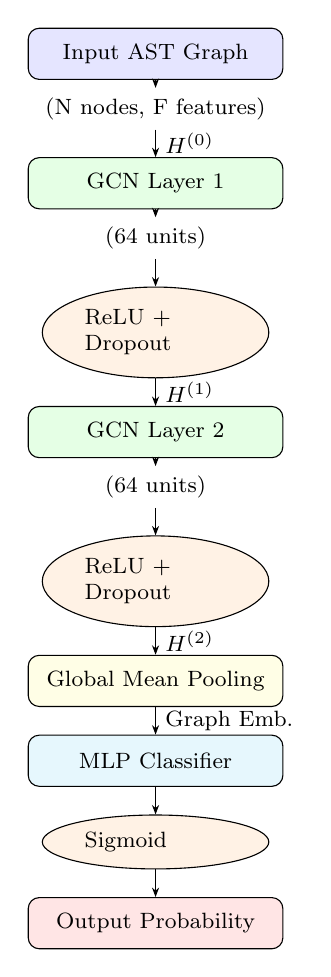
\begin{tikzpicture}[
      node distance=3.5mm, % Further reduced distance
      block/.style={rectangle, draw, fill=blue!10, text centered, rounded corners, minimum height=6.5mm, text width=30mm, font=\footnotesize},
      gcn/.style={rectangle, draw, fill=green!10, text centered, rounded corners, minimum height=6.5mm, text width=30mm, font=\footnotesize},
      pool/.style={rectangle, draw, fill=yellow!10, text centered, rounded corners, minimum height=6.5mm, text width=30mm, font=\footnotesize},
      mlp/.style={rectangle, draw, fill=cyan!10, text centered, rounded corners, minimum height=6.5mm, text width=30mm, font=\footnotesize},
      output/.style={rectangle, draw, fill=red!10, text centered, rounded corners, minimum height=6.5mm, text width=30mm, font=\footnotesize},
      ops/.style={ellipse, draw, fill=orange!10, minimum size=5mm, font=\footnotesize, text width=18mm},
      line/.style={draw, -{Stealth[length=1.2mm]}}
  ]
      % Nodes - Arranged vertically with tighter spacing
      \node (input) [block] {Input AST Graph};
      \node (input_dim) [font=\footnotesize, below=1mm of input] {(N nodes, F features)};
      
      \node (gcn1) [gcn, below=of input_dim] {GCN Layer 1};
      \node (gcn1_dim) [font=\footnotesize, below=1mm of gcn1] {(64 units)};
      
      \node (ops1) [ops, below=of gcn1_dim] {ReLU + Dropout};
      
      \node (gcn2) [gcn, below=of ops1] {GCN Layer 2};
      \node (gcn2_dim) [font=\footnotesize, below=1mm of gcn2] {(64 units)};
      
      \node (ops2) [ops, below=of gcn2_dim] {ReLU + Dropout};
      
      \node (pooling) [pool, below=of ops2] {Global Mean Pooling};
      
      \node (mlp_block) [mlp, below=of pooling] {MLP Classifier};
      
      \node (ops3) [ops, below=of mlp_block] {Sigmoid};
      
      \node (output_node) [output, below=of ops3] {Output Probability};
  
      % Connections with annotations on the right
      \path [line] (input) -- (input_dim);
      \path [line] (input_dim) -- node[right, font=\footnotesize] {$H^{(0)}$} (gcn1);
      \path [line] (gcn1) -- (gcn1_dim);
      \path [line] (gcn1_dim) -- (ops1);
      \path [line] (ops1) -- node[right, font=\footnotesize] {$H^{(1)}$} (gcn2);
      \path [line] (gcn2) -- (gcn2_dim);
      \path [line] (gcn2_dim) -- (ops2);
      \path [line] (ops2) -- node[right, font=\footnotesize] {$H^{(2)}$} (pooling);
      \path [line] (pooling) -- node[right, font=\footnotesize] {Graph Emb.} (mlp_block);
      \path [line] (mlp_block) -- (ops3);
      \path [line] (ops3) -- (output_node);
  \end{tikzpicture}
  \caption{Detailed GCN Model Architecture.}
  \label{fig:gcn_architecture}
  \end{figure}

The model takes the AST graph with its node features as input. It consists of two GCN layers (using Equation~\ref{eq:gcn}) with ReLU activations and Dropout for regularization. These layers learn node embeddings that capture local and neighborhood information within the AST. A global mean pooling layer then aggregates these node embeddings into a single fixed-size vector representing the entire graph. This graph embedding is fed into a Multi-Layer Perceptron (MLP) classifier (whose specific structure, e.g., number of layers and hidden units, is determined by hyperparameter tuning) which uses ReLU activations in hidden layers and Dropout. The final output layer uses a Sigmoid activation function to produce a probability score between 0 (likely Trojan-free) and 1 (likely Trojan-infected). The model is trained end-to-end using a binary cross-entropy loss function.

\section{Experimental Setup}
\subsection{Dataset}
The experiments were conducted using hardware designs derived from the TrustHub benchmark suite~\cite{TrustHub}. This dataset was prepared by merging the sub-module Verilog files for each selected TrustHub IP into a single \texttt{topModule.v} file. These merged designs were then categorized into Trojan-free (TjFree) and Trojan-infected (TjIn) sets. The dataset composition is present in Table~\ref{tab:dataset_summary}.
% \begin{itemize}
%     \item \textbf{Total Circuits}: 43 processed designs derived from TrustHub IPs.
%     \item \textbf{TjFree Designs (Clean)}: 9 circuits (20.9\% of the dataset). Includes processed versions of IPs such as \texttt{det\_1011}, \texttt{PIC16F84}, \texttt{RC5}, \texttt{RC6}, \texttt{RS232}, \texttt{spi\_master}, \texttt{syncRAM}, \texttt{vga}, and \texttt{xtea}.
%     \item \textbf{TjIn Designs (Trojan-infected)}: 34 circuits (79.1\% of the dataset). Consists of Trojan-inserted versions of various TrustHub IPs, including multiple variants of AES (e.g., \texttt{AES-T100} to \texttt{AES-T2100}), PIC16F84 (e.g., \texttt{PIC16F84-T100} to \texttt{PIC16F84-T400}), RS232 (e.g., \texttt{RS232-T100} to \texttt{RS232-T901}), and \texttt{wb\_conmax}.
% \end{itemize}

\begin{table}[htbp]
  \caption{Processed TrustHub Dataset Summary}
  \label{tab:dataset_summary}
  \begin{tabular}{lp{4.8cm}}
    \toprule
    \textbf{Category} & \textbf{Description} \\
    \midrule
    Total Circuits & 43 processed designs derived from TrustHub IPs \\
    \midrule
    TjFree Designs & 9 circuits (20.9\% of dataset)\\
    (Clean) & Includes: \texttt{det\_1011}, \texttt{PIC16F84}, \texttt{RC5}, \texttt{RC6}, \texttt{RS232}, \texttt{spi\_master}, \texttt{syncRAM}, \texttt{vga}, \texttt{xtea} \\
    \midrule
    TjIn Designs & 34 circuits (79.1\% of dataset)\\
    (Trojan-infected) & Includes variants of: AES (\texttt{T100-T2100}), PIC16F84 (\texttt{T100-T400}), RS232 (\texttt{T100-T901}), \texttt{wb\_conmax} \\
    \bottomrule
  \end{tabular}
  \vspace{-2mm}
\end{table}

The Trojans present in the TjIn set, originating from TrustHub, vary in type, trigger mechanism, and payload. The resulting dataset used for training is relatively small and exhibits class imbalance, with significantly more Trojan-infected samples than Trojan-free ones. This imbalance is addressed during training using oversampling and weighted loss, as detailed later. 

% Table~\ref{tab:dataset_summary} summarizes the composition of the processed dataset used in this study.

% \begin{table}[htbp] % Changed placement specifier
%   \caption{Processed TrustHub Dataset Summary} % Updated caption
%   \label{tab:dataset_summary}
%   \begin{tabular}{lcc}
%     \toprule
%     Category & Number of Samples & Percentage \\
%     \midrule
%     TjFree (Clean) & 9 & 20.9\% \\
%     TjIn (Trojan-Infected) & 34 & 79.1\% \\
%     \midrule
%     \textbf{Total} & \textbf{43} & \textbf{100\%} \\
%   \bottomrule
% \end{tabular}
% \end{table}

\subsection{Implementation Details}
\subsubsection{AST Graph Generation}
Verilog files were parsed using the `pyverilog` library. An AST generator script traversed the parsed Verilog constructs to build a graph representation using the `networkx` library. Each node in the graph corresponds to a Verilog construct, and edges represent parent-child relationships in the AST. Node features, including one-hot encoded type, depth, number of children, and average child type ID, were extracted.

\subsubsection{GCN Implementation}
The GCN model was implemented using PyTorch Geometric. The model typically consisted of two GCN layers with ReLU activation and dropout, followed by a global mean pooling layer and an MLP classifier with a sigmoid output.

\subsubsection{Training Procedure}
The dataset was split into training and testing sets using Stratified K-Fold cross-validation (with K=3 folds in the reported experiments). Oversampling was applied to the training data to handle class imbalance between Trojan-free and Trojan-infected samples. The model was trained using the Adam optimizer and a binary cross-entropy loss function with weights to account for class imbalance.

\subsection{Evaluation Metrics}
The performance of the model was evaluated using standard classification metrics, defined in Table~\ref{tab:eval_metrics}. These metrics provide a comprehensive view of the model's ability to distinguish between Trojan-free and Trojan-infected designs.

% Use table* for two-column span
\begin{table*}[ht] % Use table* and [ht] for placement suggestion - Keep as [ht] for table*
  \caption{Evaluation Metrics}
  \label{tab:eval_metrics}
  \centering
  % Use standard tabular with adjusted paragraph width for two columns
  \begin{tabular}{llp{12cm}} % Adjust p{} width as needed for two columns
    \toprule
    \textbf{Metric} & \textbf{Formula} & \textbf{Description (Context: Trojan Detection)} \\
    \midrule
    Accuracy & $\frac{TP+TN}{TP+TN+FP+FN}$ & Overall proportion of designs (Trojan or Clean) correctly classified. \\
    \addlinespace
    Precision & $\frac{TP}{TP+FP}$ & Of all designs predicted as Trojan-infected, the proportion that actually are Trojan-infected. High precision means few clean designs are misclassified as Trojan-infected (low false alarms). \\
    \addlinespace
    Recall & $\frac{TP}{TP+FN}$ & Of all actual Trojan-infected designs, the proportion that were correctly identified (Sensitivity). High recall means few Trojan-infected designs were missed (low false negatives). \\
    \addlinespace
    F1 Score & $2 \times \frac{Precision \times Recall}{Precision + Recall}$ & Harmonic mean of Precision and Recall, balancing the trade-off between missing Trojans (low recall) and false alarms (low precision). \\
    \bottomrule
  \end{tabular} % Use end tabular
  \vspace{2pt} % Add a little space after the table
  \footnotesize{$TP$: Trojan design correctly identified, $TN$: Clean design correctly identified, $FP$: Clean design misidentified as Trojan, $FN$: Trojan design misidentified as Clean.}
\end{table*} % Use end table*

\subsection{Hyperparameter Optimization}
Hyperparameters for the GCN model and the MLP classifier were tuned using Optuna, an automatic hyperparameter optimization framework. The optimization process aimed to maximize the average F1 score across the cross-validation folds. Parameters tuned included learning rate, GNN dropout rate, classifier hidden dimensions, number of classifier layers, and classifier dropout rate.

\section{Results and Analysis}
\subsection{Hyperparameter Optimization Results}
The Optuna framework was employed to search for optimal hyperparameters over 5 trials, maximizing the average F1 score across 3 cross-validation folds. The best performing set of hyperparameters identified is shown in Table~\ref{tab:best_hyperparams}. These parameters were used for the final model evaluation reported in subsequent sections.

\begin{table}[htbp] % Changed placement specifier
  \caption{Best Hyperparameters Found by Optuna}
  \label{tab:best_hyperparams}
  \centering
  \begin{tabular}{lr}
    \toprule
    Hyperparameter & Optimal Value \\
    \midrule
    Classifier Hidden Dimension & 32 \\
    Classifier Layers & 4 \\
    Classifier Dropout Rate & 0.217 \\
    GNN Dropout Rate & 0.621 \\
    Learning Rate & 0.00345 \\
  \bottomrule
\end{tabular}
\end{table}

\subsection{Cross-Validation Performance}
Using the best hyperparameters, the GCN model was evaluated using 3-fold cross-validation. The performance metrics for each fold and the average performance are summarized in Table \ref{tab:cv_results}.

\begin{table}[htbp] % Changed placement specifier
  \caption{Cross-Validation Performance Metrics}
  \label{tab:cv_results}
  \begin{tabular}{lcccc}
    \toprule
    Fold & Accuracy & Precision & Recall & F1 Score \\
    \midrule
    Fold 1 & 0.9333 & 0.9231 & 1.0000 & 0.9600 \\
    Fold 2 & 0.7143 & 0.7692 & 0.9091 & 0.8333 \\
    Fold 3 & 1.0000 & 1.0000 & 1.0000 & 1.0000 \\
    \midrule
    \textbf{Average} & \textbf{0.8825} & \textbf{0.8974} & \textbf{0.9697} & \textbf{0.9311} \\
  \bottomrule
\end{tabular}
\end{table}

The model achieved an average F1 score of 0.9311, indicating a strong ability to detect hardware Trojans. The average test accuracy was 0.8825, and the average train accuracy was 0.8976. While there was some variation across folds, particularly in Fold 2, the overall performance demonstrates the robustness of the GCN-on-AST approach. 

\subsection{Training Dynamics}
The model was trained for 200 epochs per fold. The computational efficiency, averaged over the 3 folds, is summarized in Table~\ref{tab:timing}. 

\begin{table}[htbp] % Changed placement specifier
  \caption{Computational Efficiency (Averaged)}
  \label{tab:timing}
  \centering
  \begin{tabular}{lr}
    \toprule
    Metric & Average Time \\
    \midrule
    Training Time per Fold & $\sim$20.5 seconds \\
    Training Time per Sample & $\sim$0.45 seconds \\
    Inference Time per Fold & $\sim$0.02 seconds \\
    Inference Time per Sample & $\sim$0.0013 seconds \\
  \bottomrule
\end{tabular}
\end{table}

\subsection{Comparison with Baseline Methods}
To contextualize our results, we compare the performance of our GCN-on-AST approach with reported results from the HW2VEC method~\cite{HW2VEC} applied to RTL designs, using both Data Flow Graph (DFG) and AST representations. Table~\ref{tab:baseline_comparison} summarizes this comparison.

\begin{table}[htbp]
  \caption{Comparison with HW2VEC Baseline}
  \label{tab:baseline_comparison}
  \centering
  \begin{tabular}{lccc}
    \toprule
    Method & Precision & Recall & F1 Score \\
    \midrule
    HW2VEC (DFG RTL) & 0.873 & 0.986 & 0.926 \\
    HW2VEC (AST RTL) & 0.903 & 0.800 & 0.845 \\
    \midrule
    \textbf{Our GCN (AST RTL)} & \textbf{0.897} & \textbf{0.970} & \textbf{0.931} \\
  \bottomrule
\end{tabular}
\end{table}

Our GCN-on-AST approach achieves a slightly higher F1 score (0.931) compared to HW2VEC using DFG (0.926) and significantly outperforms HW2VEC using AST (0.845). While our precision (0.897) is slightly lower than HW2VEC-AST (0.903) but higher than HW2VEC-DFG (0.873), our recall (0.970) is substantially higher than HW2VEC-AST (0.800) and comparable to HW2VEC-DFG (0.986). 

% This suggests our method is particularly effective at identifying most of the actual Trojans (high recall) while maintaining a good balance with precision, leading to the best overall F1 score among the compared methods on this dataset representation.

\section{Discussion}
The experimental results demonstrate the effectiveness of using GCNs on AST representations for hardware Trojan detection. The high average F1 score of 0.9311 achieved on the processed TrustHub dataset suggests that the model can accurately identify Trojan-infected designs while maintaining a good balance between precision and recall. 

However, several limitations should be acknowledged. The dataset used, while derived from TrustHub, is relatively small (43 designs) and imbalanced, which might limit the generalizability of the findings to larger, more complex industrial designs or different Trojan types not represented. The performance variation observed across cross-validation folds (particularly the lower F1 score in Fold 2) suggests potential sensitivity to specific data splits or overfitting, warranting further investigation with larger datasets. Finally, while GCNs achieve high accuracy, interpreting their decisions remains challenging, making it difficult to pinpoint the exact features or subgraphs indicative of a Trojan. Addressing these limitations, particularly through evaluation on more extensive datasets and the application of GNN explanation techniques, constitutes important avenues for future research.

\section{Conclusion and Future Work}
This report presented a GCN-based approach for hardware Trojan detection using AST representations of RTL Verilog code. Our method successfully leverages the structural and semantic information captured by ASTs to train a GCN model that can effectively distinguish between Trojan-free and Trojan-infected designs. Experiments on a processed dataset derived from TrustHub benchmarks demonstrated high F1 scores, highlighting the promise of this technique for automated hardware security analysis at the RTL.

Future work will focus on several directions to build upon these findings. Evaluating the approach on larger and more diverse datasets. Exploring enhanced feature engineering techniques for AST nodes and investigating more advanced GNN architectures, such as Graph Attention Networks (GATs) or Graph Isomorphism Networks (GINs), could potentially improve performance and robustness. Additionally, applying GNN interpretability methods is essential for understanding the model's decision-making process. 

%%
%% The next two lines define the bibliography style to be used, and
%% the bibliography file.
\bibliographystyle{ACM-Reference-Format}
\bibliography{sample-base} % You will need to create a sample-base.bib file or use your own



% Add a citation for TrustHub if not already present
% Example (replace with actual TrustHub reference):
% @misc{TrustHub,
%   author = {{Trust-Hub Contributors}},
%   title = {{Trust-Hub: A Benchmark Suite for Hardware Security and Trust}},
%   howpublished = {\url{https://trust-hub.org/}},
%   year = {Accessed: 2024} % Or publication year if available
% }

\end{document}
\endinput
%%
%% End of file `hardware_trojan_detection_gcn_ast.tex'.
